%
% Template for Doctoral Theses at Uppsala 
% University. The template is based on    
% the layout and typography used for      
% dissertations in the Acta Universitatis 
% Upsaliensis series                      
% Ver 5.2 - 2012-08-08                  
% Latest version available at:            
%   http://ub.uu.se/thesistemplate            
%                                         
% Support: Wolmar Nyberg Akerstrom        
% Thesis Production           
% Uppsala University Library              
% avhandling@ub.uu.se                          
%                                         
%%%%%%%%%%%%%%%%%%%%%%%%%%%%%%%%%%%%%%%%%%%


\documentclass{UUThesisTemplate}

% Package to determine wether XeTeX is used
\usepackage{ifxetex}

\ifxetex
	% XeTeX specific packages and settings
	% Language, diacritics and hyphenation
	\usepackage[babelshorthands]{polyglossia}
	\setmainlanguage{english}
	\setotherlanguages{swedish}

	% Font settings
	\setmainfont{Times New Roman}
	\setromanfont{Times New Roman}
	\setsansfont{Arial}
	\setmonofont{Courier New}
\else
	% Plain LaTeX specific packages and settings
	% Language, diacritics and hyphenation
    % Use English and Swedish languages. 
	\usepackage[swedish,english]{babel} 

	% Font settings
	\usepackage{type1cm}
	\usepackage[utf8]{inputenc}
	\usepackage[T1]{fontenc}
	\usepackage{mathptmx}

	
	% Enable scaling of images on import
	\usepackage{graphicx}
\fi


% Tables
\usepackage{booktabs}
\usepackage{tabularx}

% Document links and bookmarks
\usepackage{hyperref} 

% Numbering of headings down to the subsection level
\numberingdepth{subsection}

% Including headings down to the subsection level in contents
\contentsdepth{subsection}


% Uncomment to use a custom abstract dummy text
%\abstractdummy{
%	\begin{abstract}
%		Please use no more than 300 words and avoid mathematics or complex script.
%	\end{abstract}
%}

%Beginning of my packages
\usepackage{bibentry}
\usepackage[square]{natbib}
\usepackage{bibentry}
\nobibliography*
\usepackage{lingmacros}
\newcommand{\mn}[1]{\textbf{#1}}
\newcommand{\key}[1]{\textit{#1}}
\newcommand{\keydef}[1]{\textit{#1}}
\newcommand{\keyn}[1]{#1}
\usepackage{amssymb}

\usepackage{multirow}
\usepackage{booktabs}
\usepackage{color}

\usepackage{footnote}
\usepackage{array}
\usepackage{expex}
\newcommand{\nnumsentence}[1]{\ex<simplest>#1\xe}

\usepackage{cleveref}
\newcommand{\Eref}[1]{Example~\ref{#1}}
\newcommand{\Pref}[1]{Paper~\ref{#1}}
\usepackage{lineno}
%\linenumbers

\usepackage{tikz}
\usepackage{rotating}
\usepackage{tabularx}
\usepackage{multirow}
\usepackage{array}
\usepackage{calc}
%\usepackage{here}
\usepackage{float}
\usepackage{footnote}
%remettre package apres proof read
\usepackage{setspace}
\doublespace
%%\usepackage{doublespace}
\usepackage{footmisc}
\renewcommand\footnotelayout{\fontsize{10}{25}\selectfont}

 \usepackage{epigraph}
 % \renewcommand{\epigraphrule}{0pt}
    \renewcommand\textflush{flushright}

    \usepackage{etoolbox}
    \makeatletter
    \newlength\epitextskip
    \pretocmd{\@epitext}{\em}{}{}
    \apptocmd{\@epitext}{\em}{}{}
    \patchcmd{\epigraph}{\@epitext{#1}\\}{\@epitext{#1}\\[\epitextskip]}{}{}
    \makeatother

    \setlength\epigraphrule{0pt}
    \setlength\epitextskip{2ex}
    \setlength\epigraphwidth{.8\textwidth}



%End of my packages
\begin{document}
\frontmatter
    % Creates the front matter (title page(s), abstract, list of papers)
    % for either a Comprehensive Summary or a Monograph.
    % Authors of Comprehensive Summaries use this front matter 
    \frontmatterCS 
    % Monograph authors use this front matter 
    %\frontmatterMonograph 
 
   % Optional dedication
   %\dedication{Dedicated to all hard-working \\doctoral students at Uppsala University}
 
    % Environment used to create a list of papers
    \begin{listofpapers}
        \item  \bibentry{dubremetz2015}. \label{paper1}
        \item \bibentry{dubremetz2016}. \label{paper2}
    	\item \bibentry{Dubremetz2017}.  \label{paper3}
    	\item \bibentry{Dubremetz2018} \label{paper4}
    \end{listofpapers}
    
    
    \begingroup
        % To adjust the indentation in your table of contents, uncomment and enter the widest numbers for each level
        %  E.g.  \settocnumwidth{widest chapter number}{widest section number}{widest subsection number}...{...}
       %  \settocnumwidth{5}{4}{5}{3}{3}{3}
        \tableofcontents
    \endgroup
    
    % Optional tables
    %\listoftables
    %\listoffigures

\mainmatter
    % This includes the "Instruction", "Problem and Solutions" and "Example" files. After reading it, remove it from Thesis.tex. 
    %\input{Example/Instruction.tex}
    %\input{Example/ProblemsAndSolutions}
    %\input{Example/Example.tex}
    
    % Include your chapters here.
    \input{chapters/Abstract.tex}
    %\documentclass{UUThesisTemplate}
%\begin{document}
\chapter*{Acknowledgements}%
First and foremost, I am very grateful to my main advisor Joakim Nivre, who has taken an active interest in my work. I am grateful for his patience and his immense knowledge of natural language processing which, taken together, make him a brilliant mentor. 
 I am also grateful to my assistant advisors, Marcel Cori and Mats Dahllöf, for their thoughtful guidance.
 
Special thanks are due to my current and former colleagues in the computational linguistics group for their support, scholarly interaction, kind messages, and company throughout the years. Special acknowledgements go to Fabienne Cap, Christian Hardmeier, Sara Stymne, Aaron Smith, Miryam de Lhoneux, Beáta Megyesi, Gongbo Tang, Yan Shao, Ali Basirat, Eva Pettersson, Nils Blomqvist, Mojgan Seraji, Oscar Täckström, and Mattias Nilsson. 

My gratitude also goes to all the other members of the department for sharing meals, coffees, choir sessions or simply a good discussion. I would especially like to thank: Heinz Werner Wessler, Christer Henriksén, Karin Koltay, Eric Cullhed, Michael Dunn, Jakob Andersson, Helena Löthman, Johan Heldt, Christian Schaefer, and Harald Hammarström.  

I also address my deep thanks and encouragement to all the other PhD fellows at the department, namely Rima Haddad, Josefin Lindgren, Alexander Nilsson, Marc Tang,  Linnéa Öberg, Vera Wilhelmsen, Jaroslava Obrtelova, Fredrik Sixtensson, Myrto Veikou, Emil Lundin, Samuel Douglas, Mahmut Agbaht, Buket Öztekin, who contributed to making my workplace a nice place to be.

I would further like to thank the administrative and technical staff of Uppsala University for their support and professionalism, in particular Per Starbäck, Inga-Lill Holmberg, Jenny Rahbek and Ina Sörlid.


I am grateful to my friends, both in Lille and Uppsala. Thank you for staying by my side, even at times when I neglected you for the sake of my research.  

Last, but not least, without my dear family I would never have completed this work. Thank you! You should know that your support and encouragement was worth more than I can express in writing.

        %\documentclass{UUThesisTemplate}
%\begin{document}
\chapter{Introduction}%
\epigraph{If a man will begin with certainties, he shall end in doubts; but\\ if he will be content to begin with doubts, he shall end in certainties.}{--- Francis Bacon}
%In this thesis we are interested in repetitions of words.  Indeed,
\noindent
Language is full of repetitions of words. %It is a statistical fact: we have a limited vocabulary and few words of our vocabulary are used frequently. %\citep{Zipf1936}. 
While reading this text, you have already encountered several of them without noticing it. And, in fact, it is normal; % to not pay attention to them:
 they are not an interesting event for our mind. 
However, sometimes we meet exceptions, %those exemptions are the object of this thesis. And some example of them are contained
% 
like
  in the following text:
\begin{quotation}
%``And as wondrous as it is, it cannot be reduced to a kind of simplification that we have often come to be admired. 
And yet, as wondrous as it is, our lives are complex. 
Our emotions are complex. 
Our intellectual desires are complex.  
%So I do believe that architecture as I see it needs to mirror that complexity in every single space that we have, in every intimacy that we possess. 

 When it comes to complexity there is no short term fix in a pill. % or anything else. 
%But
And your friends are long-term supports, and therefore, perhaps the most significant thing you can do to add more years to your life, and life to your years. %''
\end{quotation}

%You just came across some examples of rhetorical effects built with those uncommonly noticeable repetitions that create what we call \key{figures of speech}. 
\noindent
In this text, the repetition of the word ``complex'' three times, and the words ``life'' and ``years'' twice, probably caught your attention, or at least they caught your attention more than the repetition of the word ``as'' at the beginning of the text. %If you have to translate or read this text out loud, you will have to take into account this effect. We call such noticeable effect a figure of speech and when it involves a repetition we call it figure of repetition. 
We may not be conscious of making such a hierarchy in our attention to repetitions, but it is nevertheless an important part of our ability to correctly analyse, translate or read this text out loud in the most natural way. The authors of antiquity already knew about the properties of certain types of repetitions and included them in a subcategory of figures of speech which we call the figures of repetition. In this thesis we focus on three of them.
\bigskip

\noindent \key{Chiasmus},
%\footnote{The term comes Greek letter $\chi$ because of the cross this letter symbolises (see Figure~\ref{graphX} %======Schéma=======
%\begin{figure}[h!] 
%\begin{center}
%\includegraphics[scale=0.45]{images/X}
%\caption{Schema of a chiasmus.}
%\label{graphX}
%\end{center}
%\end{figure}
%%======Schéma=======).
%
%}
 which is the repetition of a pair of words in reverse order such as \Eref{ex:Mountain}.
%
\nnumsentence{If the \mn{mountain} won't come to \mn{Muhammad},\\ then \mn{Muhammad} must go to the \mn{mountain}. \label{ex:Mountain}}%
%

\noindent\key{Epanaphora}, the repetition of one or several words at the beginning of sentences as in \Eref{ex:Mylife}.%
%
\nnumsentence{\mn{My life is my} purpose.\\ 
\mn{My life is my} goal. \\
\mn{My life is my }inspiration. \label{ex:Mylife}}%
%
\noindent\key{Epiphora}, the repetition of one or several words at the end of the text, like in \Eref{ex:War}.
\nnumsentence{The United States, as the world knows, will never start \mn{a war}.\\
We do not want \mn{a war}.\\
We do not now expect \mn{a war}.\label{ex:War}}%
%
\vspace{-28pt}
\section{Research Questions and Contributions}

For a computer, locating all repetitions of words is trivial, but locating just those repetitions that achieve a rhetorical effect is not. Can this distinction be made automatically? The methods and models presented in this thesis focus on \textit{how} a computer can detect those figures of repetition. 
\begin{enumerate}
\item How should we define the task for detection of figures of repetition?
\item  What challenges are posed by different types of figures with respect to features and machine learning?

\item Can we automatically learn how to weight different features, and how much manually annotated data do we need for that?
\item How do we evaluate the performance on this task?
\item Which types of linguistic features are useful?
% \item To what extent can we distinguish rhetorical from accidental repetitions using automatically extracted linguistic features?
% \item Which types of linguistic features are useful?
% \item Can we automatically learn how to weight different features given the small amounts of annotated data?
%  \item  What challenges are posed by different types of figures with respect to features and machine learning?


\end{enumerate}
The main contributions of this thesis are:
\begin{enumerate}
\item A general model for detecting repetitive rhetorical figures, including a method of evaluation.
\item An experimental evaluation of this model with respect to chiasmus, epa\-naphora and epiphora, exploring the usefulness of different features and comparing machine learning and hand-tuning of feature weights.
\item A pilot study comparing the frequency of different figures in different text genres.
\item The development and testing of three systems of detection designed for the three repetitive figures we are looking for.
\item A number of corpora annotated for chiasmus, epanaphora and epiphora.
\end{enumerate}
\section{Outline of the Thesis}
%The outline of the thesis is as follow. 
%\bigskip

%\noindent Chapter 2 provides the motivation for studying the detection of repetitive figures. Through examples we will see that repetitive figures present a scientific interest from both a linguistic and computational linguistic point of view. We motivate the method used. Finally we explain why we focus on detection and not on generation.
%\bigskip

\noindent  Chapter 2 presents background information about figures of speech in general, and how they are split into categories. We describe the state of the art for their treatment in computational linguistics.
\bigskip

\noindent  Chapter  3 introduces the general method we use for all of our repetitive figure detectors. We will explain the model used for ranking, the evaluation method, the annotation process, and the tuning process. 
\bigskip

\noindent  Chapter 4 summarises the empirical results of our experiments. We analyse the performance of each system and discuss its statistical significance.
\bigskip


\noindent Chapter 5 summarises the contributions of the thesis. We conclude with a discussion of promising directions for future research.
\bigskip

\noindent  Chapter 6 provides a brief overview of the papers included in this thesis.

%\normalsize

%In Paper~\ref{pc} we show
%\includegraphics[scale=1]{X}
%\end{document}
    %\documentclass{UUThesisTemplate}
%\begin{document}
%CECI est un CITE \cite{Butler1921}\\
%CECI est un CITEp \citep{Butler1921}\\
%CECI est un CITEt \citet{Butler1921}\\
%\\
%CECI est un CITE \cite[p.1]{Butler1921}\\
%CECI est un CITEp \citep[p.1]{Butler1921}\\
%CECI est un CITEt \citet[p.1]{Butler1921}\\
\chapter{\label{chap3}Background}%
This chapter provides background information on rhetoric, rhetorical figures and our three figures of speech from the perspective of literary analysis and computational linguistics. This review does not attempt to cover all relevant issues and is by no means exhaustive. Instead, we focus the discussion primarily on aspects that have some bearing on Papers~I–IV.

\section{Rhetoric}
One cannot talk about figures of speech without invoking their antique theoretical framework. The concepts for the figures of speech have their historical roots in the field of rhetoric, whose aim is to teach speakers to convince and persuade their audience. 
The most fundamental notions of rhetoric were defined by Aristotle \citep{Roberts2004} as follows:

\begin{quotation}
Of the modes of persuasion furnished by the spoken word, there are three kinds. The first kind depends on the personal character of the speaker [ethos]; the second on putting the audience into a certain frame of mind [pathos]; the third on the proof, or apparent proof, provided by the words of the speech itself [logos]. Persuasion is achieved by the speaker’s personal character when the speech is so spoken as to make us think him credible.
   –Aristotle 1356a 2,3 (Translated by \cite{Roberts2004})
\end{quotation}
\noindent
In this extract, Aristotle gives three key notions to explain the mechanisms involved when trying to persuade someone. One can act on the ethos, which is the way one gives credit to the speaker. Then one can act on the pathos, that is, the appeal to the emotion of the audience. Finally one can act on the logos, which in Greek means both logic and discourse, and which can be defined as the way one articulates the ideas, the reasoning. While Aristotle preferred that arguments be based as much as possible on logos, he did pay considerable attention to the appeal to emotion, and discussed it extensively in his \textit{Rhetoric}.


Ancient authors such as Hermogenes and Quintilian \citep{Butler1921} were passionate about rhetoric and not only practised it but also tried to define and model it. They observed patterns of discourse that would benefit their argumentation. Among those patterns are the ornaments called figures of speech, also known as rhetorical figures. In his Oratio  \citep{Butler1921} Quintilian tries to describe all the figures. His classification still inspires works of classification today \citep{harris2009,Burton1996}. This classification is not uncontroversial.  Indeed, the notion that figures of speech are additional ornaments that deviate from a ``normal'' way to express things has been repeatedly questioned in modern linguistics and philosophy \citep{Jakobson1956,Derrida1982}.%[white mythology]
 
 Figures of speech can, in fact, leverage any of the appeals identified by Aristotle (logos, pathos, ethos). In an extensive work of classification, \cite{Howard2010} tries not only to define each figure of speech but also to label them with the appeal they are used for. For instance, he says that chiasmus and epanaphora appeal to logos and pathos. That can be a subject of controversy. For instance, \citet{Vandendorpe1991} seems to criticise some examples of chiasmi for acting merely on the impression made by the author, and by extension the ethos. Indeed, for him, this figure is an over-sophisticated way to express what sometimes are very cliché ideas (for example, ``the research of the meaning is the meaning of research''). Thus, for \citet{Vandendorpe1991}, this extreme ability to play with words could make the audience give too much credit to the speaker by thinking that he or she is clever. As we will see in \Cref{secDef}, rhetorical figures are vaguely defined, and this is just one example of the controversies raised by this topic.

% In distinguishing schēma from trope, Quintilian calls it “a purposeful deviation in sense or language from the ordinary simple form; the analogy is now with sitting, bending forwards, or looking back” ( Institutio oratoria . Later analogies reinforce this distinction between inward meaning and outward form by comparing schemes to costume, clothing, and ornament. Cl. definitions of scheme thus rely on an idea of ordinary (naked, natural, or plain) speech that is then clothed by the figures of rhet. The discursive force of such *ornament varies throughout rhet.’s long hist., with schemes swelling in number and acquiring greater currency in courtly cultures that emphasize fashion, performance, or external show as constitutive of identity. In theories of rhet. and poetics informed by mod. ling., there is considerable skepticism toward the notion that there exists an “ordinary” lang. to be ornamented by figures of speech. Such theory concludes that rhetorical figures are not supplementary decorations but rather fundamental structures of lang. and thought ( Jakobson, Derrida, de Man). Although this theory of figures as constitutive of, and coextensive with, lang. makes its exemplary arguments with reference to tropes such as *metaphor and *metonymy, it has resulted in a generalized critical method inclined to discover substantive meaning in the lexical patterns and shapes of what used to be called rhetorical schemes. See figuration, linguistics and poetics, rhetoric and poetry. ᭿ Jakobson and Halle, “Two Aspects of Language and Two Types of Aphasic Disturbances”; E. Auerbach, “Figura,” trans. R. Manheim, Scenes from the Drama of European Literature (); O. Ducrot and T. Todorov, Encyclopedic Dictionary of the Sciences of Language , trans. C. Porter (); G. Genette, Figures of Literary Discourse , trans. A. Sheridan (); T. Todorov, Introduction to Poetics , trans. R. Howard (); de Man, “The Rhetoric of Temporality” and “The Rhetoric of Blindness”; P. de Man, “Anthropomorphism and Trope in the Lyric,” The Rhetoric of Romanticism (), and “Hypogram and Inscription” and “The Resistance to Theory,” The Resistance to Theory (); J. Derrida, “White Mythology,” Margins of Philosophy , trans. A. Bass (); Vickers, Defence ; B. Dupriez, A Dictionary of Literary Devices (); Lanham; Renaissance Figures of Speech , ed. G. Alexander, S. Anderson, and K. Ettenhuber (); G. Burton, “Silva Rhetoricae,” http://rhetoric. byu.edu. J. C. Mann SCHOOL OF SPENSER. A group of Eng. poets of the earlier th c., strongly under the influence of Edmund Spenser (– ). Their work is sharply distinguished from the more radical poetic movements of the time, epitomized by the *classicism of Ben Jonson and the *metaphysical style of John Donne. The principal poets of the Spenserian school—William Browne of Tavistock, Michael Drayton, George Wither, Giles and Phineas Fletcher, and the Scottish poets William Drummond of Hawthornden and Sir William Alexander— show the influence of Spenser in their sensuous imagery, smooth meter, archaic *diction, and fondness for narrative and *pastoral modes of expression. They also owe to Spenser their allegorical and moral tendencies. Such ambitious narrative poems as Giles Fletcher’s Christ’s Victory and Triumph and Phineas Fletcher’s The Apollyonists suggest Spenser’s Faerie Queene in their pictorial quality and their stanza forms (modified *Spenserian stanzas); they also anticipate John Milton, who, occasionally echoing the Fletchers, followed them in the use of Christian material for epic purposes and who himself acknowledged his indebtedness to Spenser, whom he called master . ᭿ H. E. Cory, Spenser, the School of the Fletchers, and Milton (); D. Bush, English Literature in the Earlier Seventeenth Century, –  , d ed. (); J. Grundy, The Spenserian Poets (); The English Spenserians, ed. W. B. Hunter Jr. ()—anthol.; P. J. Finkelpearl, “John Fletcher as Spenserian Playwright: The Faithful Shepherdess and The Island Princess ,” SEL  (); M. Quilligan, Milton’s Spenser (); G. M. Bouchard, “Phineas Fletcher: The Piscatory Link The Princeton Encyclopedia of Poetry and Poetics : Fourth Edition, edited by Stephen Cushman, et al., Princeton University Press, 2012. ProQuest Ebook Central, .Created from uu on 2017-09-28 07:40:08. 
%Previous extract from "scheme" in greene.
% is still inspiring works on classification of today \citep{harris2009,Burton1996}. Although the all notion of figures of speech as simple additional ornament that would deviate to a somewhat `normal' way to express things is abundantly questioned by the contemporary linguistics framework \citep{Jakobson1956},\citep[White Mythology]{Derrida1982}.
 
% Figures of speech can in fact leverage any of the appeals defined by Aristotle (logos, pathos, ethos). In an extensive work of classification \cite{Howard2010} tries not only to define each figures of speech but also to label them with the appeal it is used for. For instance he says that chiasmus and epanaphora appeals to logos and pathos. That can be subject of controversies as \citep{Vandendorpe1991} seems to criticise some examples of chiasmus for acting merely on the image given by the author, so by extension the ethos. Indeed, for him, this figure is an over sophisticated way to express an idea sometimes very cliché (i.e. `The research of the meaning is the meaning of research'). Thus for \citet{Vandendorpe1991} this extreme ability to play with word could push the audience to give too much credit to the speaker by thinking that he or she is clever. As we will see in \Cref{secDef} rhetorical figures are vaguely defined and, this is just one example of controversy raised up by this topic.
 
\section{Rhetorical Figures\label{secDef}}
\subsection{Schemes and Tropes}
\keyn{Figures of speech}, also called \keyn{rhetorical figures}, are commonly divided into two categories,  \keydef{tropes} and \keydef{schemes}. This separation between figures of speech comes from the classification of Quintilian \cite[p.196]{fahnestock1999}. 

A trope is defined as:
\begin{quotation}
An artful deviation from the ordinary or principal signification of a word. \\\citep{Burton1996}%\footnote{http://rhetoric.byu.edu/Figures/Tropes.htm}
\end{quotation}
\noindent
Tropes such as “the Lord is my shepherd” (metaphor), “the pen is mightier than the sword” (metonymy), and “the face that launched a thousand ships” (synecdoche) operate by changing the signification of the words ``shepherd'', ``pen'', ``sword'', and ``face''. %Thus, tropes allow language to mean more or something new.% \citep[Art. Trope]{greene2012}. 


\cite{greene2012} define a scheme as a change in standard word order or patterns. This includes any artful deviation from the ordinary arrangement of words. Unlike tropes, which work on the signification of words, schemes involve their arrangement \citep[Art. ``Scheme'']{greene2012}.  For instance an enjambement can be considered as a scheme. It is defined as an unnatural ``cut'', which can result in stylistic effects (emphasis, contrast, double interpretations) (see \Eref{exEnjamb}).
\nnumsentence{I’d rather\\
be naked \\
of fake friends\label{exEnjamb}}%\vspace{-18pt}
%
Beneath the category of schemes, there are many subcategories. Among them are the categories of repetitive figures or figures of repetition, which include every figure involving repetition of linguistic units such as letters, words or concepts.
 This is where chiasmus, epanaphora and epiphora belong. Depending on the sources, their number can vary, as will be explained for the case of chiasmus (\Cref{secChiasmus}). As for now, we can say that there is no one unique way to name and categorise figures. We are not going to list all figures of repetition,\footnote{For an extended list of repetitive figures, we refer the reader to \url{http://rhetoric.byu.edu/Figures/Groupings/of\%20Repetition.htm}. } but we can present three clear examples that are representative of what repetitive figures can be.
 \begin{itemize}
  \item Alliteration: Repetition of initial or medial consonants in two or more adjacent words.
  \item Anadiplosis: Repetition of a word at the end of a clause and then at the beginning of the succeeding clause.
%\item Assonance: Repetition of similar vowel sounds, preceded and followed by different consonants, in the stressed syllables of adjacent words.
 \item Antanaclasis: Repetition of a word in two different senses.
 \end{itemize}
Another controversy that has some bearing on our work concerns whether a figure of speech (trope or scheme) should be considered only if it is \keydef{intentional} or, in other words, is intended by the author. Such a definition of figures of speech, used in some computational linguistics work \citep{Strommer2011}, causes a problem in the literature field.\footnote{The status of the author has been widely questioned in both 20th-century and contemporary literary theory \citep{Barthes1984}. Indeed, it is argued that no one can really pretend to know the intention of the author. We are aware of this controversy but will not address it here.} For this reason we avoid focusing too closely on the term ``intentional'' because we do not want to fall into any author fallacy. This choice will be reflected in how we formulate our questions during the annotation process (see \Cref{secHowAnnot}).  %, and it is certainly not our role to say if it is true or not.} 

%As far as we are concerned, the debate on intentionality is of limited relevance for this thesis. Indeed
%, de facto when we will annotate examples, 
%we will be dependent on what is our own interpretation as a reader. This perception can vary between annotators. Thus, we choose to avoid the term `intention' because it would suggest that we pretend to know the auctorial intention and that we limit text interpretation to what the author meant. 
%The important thing to explain here is how this can impact our task concretely. 
%this theoretical assumption, most of the time, will not significantly change the system we develop as we focus the task on detecting the most prototypical cases. After all, when someone quotes `Fool is fair and fair is fool', whether you read this sentence from the supposed point of view of the author or from the perception of the reader, the conclusion should be the same: we are in the presence of a chiasmus. It is only in some borderline cases that our theoretical position has impact. 
%%%%%%EXAMPLE REMOVED%%%%
%\footnote{Let us take this exceptional but real example extracted from a French book:
%
%\nnumsentence{he \mn{regifies} the \mn{stars} and \mn{starifies} the \mn{kings} \label{exStar}}
%
%When looking at this example, some users will never see any chiasmus. However, some others, if they have studied latin, will argue that `regifies' comes from the Latin `rex/regis' which means king;  thus there is a chiasmus playing on the notions of `king' and `star'. If we take the auctorial point of view, we will have to document ourselves and see if the author has studied latin and conclude if he/she is likely to have intended this chiasmus. However, if we abandon the idea of looking for what was the intention of the author, we can consider that this chiasmus does not exist in the eyes of most readers because most readers are non-latinist.} 
%And in reality, we will see in Chapter~4 by comparing the results of our exploration on epanaphora with the ones of \citet{Strommer2011} that we have reasons to believe that this theoretical choice does not impact dramatically the number of candidates we consider as real instances of rhetorical figures. 

In this first part, we have given a general overview of what rhetoric is and how rhetorical figures can be defined. We have touched on aspects of the theoretical debate that can be relevant to our approach to detection. In the next section, we give a definition of the three figures we are studying. One figure, however, will be studied more extensively: chiasmus. Throughout this study, we will see how multiple challenges already arise when searching for a definition and a list of terms adapted to the requirements of computational linguistics.\clearpage

\subsection{Chiasmus}
\label{secChiasmus}
The word ``chiasmus'' comes from the Greek letter $\chi$ because of the cross this letter symbolises. Indeed, chiasmus is generally defined as the reuse of a pair of elements in reverse order, as in Figure~\ref{crossSchem1}.
\vspace{0.2cm}%
\begin{figure}[H] 
\begin{center}
%\resizebox{0.1}{0.1}{
\begin{tikzpicture}[scale=1.5]
\draw [very thick]  (0,1.5) node[above]{$A$} -- (1,0.5) node[below]{$A'$};
\draw [very thick]  (0,0.5) node[below]{$B'$} -- (1,1.5) node[above]{$B$};
\end{tikzpicture}
%}
\end{center}
\vspace{-0.3cm}
\caption{The chiasmus schema \label{crossSchem1}} 
\end{figure}
\vspace{-0.5cm}
\begin{figure}[h!] 
\begin{center}
\includegraphics[scale=0.5]{images/X}
\vspace{-0.4cm}
\caption{A chiasmus example\label{graphX}}
\end{center}
\end{figure}%
\vspace{-0.1cm}
\noindent
There are many forms of chiasmus. They can consist of cross-like arrangements of phonemes, letters, or syntactic elements. We will focus on the chiasmus of words, also called antimetabole. However, even within this single subcategory, we observe many variations that we need to define for the automatic treatment \citep{gawr}. As a result of this, we present the types of chiasmus of words that we have identified.\footnote{This typology is inspired by and adapted from the one developed in French by \cite{dubremetz2013}.} This typology was obtained by reading a number of
definitions given in the literature \citep{Diderot1789,gradus,garcia,greene2012,larousse,Nordahl1971,
rabatel,Vandendorpe1991,VanGorp2001} and observing what kinds of examples they are citing.
\clearpage
%Il existe toute sorte de chiasmes, ils peuvent porter sur le croisement de phonèmes, de lettres, d'éléments syntaxiques... Nous nous restreindrons à l'étude des chiasmes de mots. Cependant on constate dans cette sous-classe de chiasmes encore beaucoup de variantes qu'il faut définir pour le traitement automatique \cite[p.67]{gawr}.  Voici donc, à l'issue des lectures des linguistes \footnote{ \citet{Diderot1789,gradus,garcia,Greene2012,Nordahl1971,larousse,rabatel,Vandendorpe1991,VanGorp2001}} et de l'observation des exemples qu'ils donnent, les types de chiasmes de mots que nous avons recensés :



%\begin{table}[H]
%\begin{savenotes}\label{tablSynthDef}
%%=============TABLEAU=========
%\begin{tabular}{|b{1.5cm}|p{2cm}|p{3cm}|p{3cm}|p{3cm}|}
%\hline
% & \multicolumn{2}{c|}{\textbf{Name}} & \textbf{Repeted Elements:} &\textbf{\ \ \ \ \ \ \  Example}\tabularnewline
%\hline 
%\hline 
%	\multirow{30}{1.5cm}{
%	\begin{center}\textbf{Chiasmi of words}%\\\\\\\
%%========FIGURE=========
%\begin{figure}[H]
%\ \ \ \begin{tikzpicture}[scale=0.4]
%\draw [very thick]  (0,1.5) node[above]{$A$} -- (1,0.5) node[below]{$A'$};
%\draw [very thick]  (0,0.5) node[below]{$B'$} -- (1,1.5) node[above]{$B$};
%\end{tikzpicture}
%%\caption{Schéma définitoire du chiasme} \label{crossSchem1}
%\end{figure}
%%========FIGURE=========
%	\end{center}} 
%
%%	%=====première entrée=====
%		 	& \multicolumn{2}{p{3cm}|}{\begin{center}Antimetabole or Strict antimetabole\end{center}} 
%		 	&\begin{center} identical words / pair of strings \footnotemark{\cite[Art."Chiasme"]{gradus, larousse}}  \end{center}
%		 	& \textit{\textit{\mn{Sounds} of \mn{poetry}, and \mn{poetry} of \mn{sounds}.}%(Shakespeare)
%		 	} \tabularnewline
%	%!=====deuxième entrée=====
%			\cline{2-5} 
%	%=====troisème entrée=====
%		 & \multicolumn{2}{p{3cm}|}{\begin{center}Flexional chiasmus or Flexional antimetabole\end{center}}  
%		 & \begin{center}
%inflected lemmas
%\end{center}
%		 & \textit{An optimist \mn{laughs} to \mn{forget}, a pessimist \mn{forgets} to \mn{laugh}.} %(Anonymous)
%		 \tabularnewline
%	%=====troisème entrée=====
%		\cline{2-5} 
%	%=====quatrième entrée=====
%		 & \multicolumn{2}{p{3cm}|}{\begin{center}Derivational chiasmus\end{center}} 
%		 & \begin{center}derived stems \end{center}
%		 &\textit{ \mn{Modernise} \mn{Islam} rather than \mn{islamisation} of \mn{modernity}.} %(Jean Daniel)
%		 \tabularnewline
%	%=====!quatrième entrée=====
%		\cline{2-5} 
%	%=====cinquième entrée=====
%		 & \multicolumn{2}{p{3cm}|}{\begin{center}Antimetalepse\end{center}} 
%		 & \begin{center}
%Idea or notion but without necessarily reusing morphologically related words \footnote{\cite[Art. "Antimétabole, Antimétalepse, Antimétathèse"]{Diderot1789}} 
%\end{center}
%		 &  Who \mn{dotes}, yet \mn{doubts}; \mn{suspects}, yet \mn{loves}.%---Othello
%		 \tabularnewline
%	%!=====cinquième entrée=====
%\hline
%\end{tabular}\end{savenotes}
%\caption{Typology of chiasmus of words\label{tabTypo}}\end{table}

%%%%%%%%%%%%%%%%%%END TABLEAU

\begin{table}[H]

\begin{savenotes}\label{tablSynthDef}
\footnotesize

%=============TABLEAU=========
\begin{tabular}{|c|c|c|}
\hline
\textbf{Name} & \textbf{Repeated Elements} &\textbf{Example} \\
\hline 
Antimetabole or & Identical word forms\footnotemark[4] & \mn{Sounds} of \mn{poetry},  \\
Strict antimetabole & (pair of strings) & and \mn{poetry} of \mn{sounds}.\\
\hline 

Flexional chiasmus or & Inflected lemmas & An optimist \mn{laughs} to \mn{forget},  \\ %(Anonymous)
Flexional antimetabole & & a pessimist \mn{forgets} to \mn{laugh}. \\
\hline 
Derivational chiasmus & Derivations with same stem & \mn{Modernise} \mn{Islam} rather than \\ %(Jean Daniel)
& & \mn{islamisation} of \mn{modernity}. \\
\hline 
Antimetalepse & Ideas or notions, but without & Who \mn{dotes}, yet \mn{doubts}; \\%---Othello
& necessarily reusing  & \mn{suspects}, yet \mn{loves}. \\
& morphologically related words\footnotemark[5] & \\
\hline
\end{tabular}\end{savenotes}

\caption{Typology of chiasmus of words\label{tabTypo}}\end{table}



\footnotetext[4]{\cite[Art."Chiasme"]{gradus, larousse}}
\footnotetext[5]{\cite[Art. "Antimétabole, Antimétalepse, Antimétathèse"]{Diderot1789}}
\setcounter{footnote}{5}


 Even if the term chiasmus is a recent one,\footnote{This term does not appear until the second half of the 19th century \cite[p. 24]{horvei1985}.} the figures described in this table are very old and have been known for a long time. For instance, already in Quintilian we observe the existence of antimetabole of identical terms but with different inflexions, though no name has ever been given to this phenomenon to differentiate it from the strict antimetabole. A similar lack of defining terms is noticeable for the chiasmi that allow derivations.
 This table is probably not exhaustive and it is dependent on the examples cited as canonical in the literature. It should not be seen as the sole possible classification of chiasmus and antimetaboles. In fact, some authors prefer to refer to antimetabole as reverted antithesis \citep{Viklund2002}. Others, by contrast, want to consider those special cases a completely different figure called ``reversion'' \cite[Art. Reversion]{font}.\footnote{We can trace this back to another conflicting classification in Antiquity, as Hermogenes prefers to place chiasmus under a category of figure completely separated from other figures of repetition. For him chiasmus belongs to ``gorgotes'' (i.e.,``vigour''), whereas epanaphora and epiphora are a sort of parallel figures that should be placed under ``kallos'' (i.e., ``beauty'') \citep{Wooten2012}.}   
 As stated by \cite[p. 3]{Watson1912}:
\begin{quotation}
 The importance attached to rhetorical expression among ancient writers is recognized not only by special treatises written by them, but in the compilations or writings on rhetoric by modern authors who have made special study of such treatises. These ancient writers discuss in bewildering profusion examples with subdivisions of tropes, figures of rhetoric, figures of syntax, etc. But frequently their definitions do not offer a basis for clear cut division. Hence it is often impossible to make any sharp or important distinction between tropes, figures rhetorical, and figures grammatical, and no two writers of the present day arrange them in exactly the same way.
\end{quotation}
\noindent
 Thus we see \Cref{tabTypo} as one possible classification that answers our specific problem of defining the task for a computer. %It will allow us to progress towards the definition of the task to be carried out by the computer. 
 Indeed without a clear, formal and adapted definition, it will be difficult to make any system of detection \cite[p. 67]{gawr}.
 
%  \cite[Art. Antimétabole]{Greene2012} l'existence des antimétaboles comportant des mots identiques mais aux flexions différentes. Cependant jamais un nom spécifique n'a été donné à ce phénomène pour le différencier de l'antimétabole stricte. Il en va de même pour le chiasme portant sur des mots dérivés.
%Ce tableau n'est sans doute pas exhaustif puisqu'il est tributaire d'observations empiriques à partir des exemples donnés par les ouvrages de stylistique de référence. Il va cependant permettre à cette recherche d'aller plus loin et de ne pas se heurter au flottement {}\cite[p.21]{rabatel} qui règne autour de la définition de cette figure : car sans définition formelle, il s'avère difficile d'élaborer un système de détection \cite[p.67]{gawr}.





%The chiasmus of words, also called antimetabole, is defined as the repetition of a pair of words in reverse order. %The term chiasmus of words, sometimes called antimetabole, consists in the reuse of a pair of words in reverse order for a rhetorical purpose. 
%It is called `chiasmus' after the Greek letter $\chi$ because of the cross 
%this letter symbolises (see Figure~\ref{graphX}).
% %======Schéma=======
%\begin{figure}[h!] 
%\begin{center}
%\includegraphics[scale=0.5]{images/X}
%\caption{Schema of a chiasmus}
%\label{graphX}
%\end{center}
%\end{figure}

From now on, we will restrict the term `‘chiasmus’' to cases based on identity of lemma  (i.e., flexional chiasmus in \Cref{tabTypo}). This restriction is a compromise aiming to make the task feasible. Indeed, if we tried to detect all kinds of chiasmus, technical difficulties would pile up  that would prevent any deep investigation. For example, the extraction process would become noisier and we would have to improve stemmers as well as ontologies \citep{dubremetz2013}.

In this part we have investigated the definition(s) of chiasmus, and have proposed a typology. This typology divides chiasmi into different subtypes based on similarities between words, and can differ from some authors' definitions partly because there is a lack of consensus about what kind of figure each name should denote. This does not however mean that we completely ignore other definitions. In fact, we consider those other definitions to be observations about the figure behaviour, which provides a precious help in designing features. For instance, in \Pref{paper1}, we decide to use negations like ``not'' in order to capture chiasmi based on antithesis. In \Pref{paper2} we decide to model switching of  syntactic roles between main words in order to model the notion of symmetry described by \cite{morier}.

When we get to the actual experimentation in this thesis, the definition of a candidate chiasmus will be limited as follows:
\bigskip
\begin{enumerate}
\item A chiasmus is the repetition of a minimum of two pairs of words in reverse order satisfying the ABB$\textprime$A$\textprime$ schema, as in \Cref{crossSchem1}.
\item The words repeated should appear within a reasonably limited context. In our actual implementation: 30 tokens.\footnote{30 tokens is the upper bound found empirically by \citet{dubremetz2013}. In that corpus study, the largest chiasmus found consisted of 23 tokens.}
\item The word pairs (AA$\textprime$ and BB$\textprime$) should have the same lemma.
\end{enumerate}
%Despite a long tradition in rhetorics and linguistics, the terms {\em chiasmus} and {\em antimetabole} do not really have clear definitions. In the earliest times, \citet{Diderot1789} as well as Quintilian \citep{Greene2012} give us very basic identification features. They talk about the degree of identity that can be accepted to consider two words as identical (strictly identical strings, lemmas or synonyms). Finally, \citet{rabatel} and \citet{Nordahl1971} try to find subcategories of chiasmi on a deep semantic basis: for instance chiasmi expressing contrast \cite{rabatel}. %The notion of antimetabole is floating. Dictionaries of stylistics tend to quote the same prototypical chiasmi to illustrate examples, which is not helpful when trying to capture the linguistic variety of chiasmi.



\subsection{Epanaphora}
The lack of definitions adapted to computational linguistics is not exclusive to chiasmus. In fact, any figure of speech suffers from a lack of consensus about the definitions, or from vagueness in delimiting what we are looking for. Epanaphora confirms this rule.
Epanaphora\footnote{In rhetoric, \emph{epanaphora} is better known under the competing term \emph{anaphora}. However, in computational linguistics the term \emph{anaphora} can be ambiguous, as it also refers to a referential pattern. For the sake of clarity, we will only use the term \emph{epanaphora}.}
 is defined as the repetition of a word or a group of words at the beginning of several sequences of language. Curiously, the ambiguity in the definition of epanaphora does not concern the same issue as for chiasmus. For chiasmus it is the type of element that can be criss-crossed (sounds, letters, strictly similar words or just synonyms) that is unclear. For epanaphora there seems to be some kind of consensus: only words should be the object of the repetition (not letters or sounds). And all examples cited by our references were concerned with repetition of words that at least share the same lemma. Where the definition gets blurry is: (1) What type of sequences should be considered? (2) How close together should they be? 

Regarding the first question, ``sequences'' can be defined in different ways. One can speak of epanaphora of paragraphs \citep[Art. L'anaphore et l'épiphore]{Bacry1992}, verses \citep[Chap. III]{Suhamy2004}, clauses or phrases \citep[Art. Anaphore]{gradus}. All authors have at least invoked or cited in their examples the sentence as a possible sequence for epanaphora production. In addition, sentence splitting is a nearly solved problem in natural language processing. Sentences should not represent a major challenge for definition and extraction. That is why, in this thesis, we limit the scope to epanaphora of sentences, as exemplified in  Example~\ref{exIam}. 
%
\nnumsentence{\mn{I am} an actor.\newline
\mn{I am} a writer.\\
\mn{I am} a producer.\\
\mn{I am }a director.\\
\mn{I am }a magician. \label{exIam}}%
%
On the second question, some authors, like \citet[Chap. III]{Suhamy2004} and \citet[Art. L'anaphore et l'épiphore]{Bacry1992}, talk about ``successive'' sequen\-ces, while others seem to consider repetitions that skip one or several sequences before producing a repetition to be an epanaphora \cite[p.329]{font}. To keep the problem simple, we will consider only epanaphora relying on immediately successive sentences.

%  \enumsentence{\mn{We shall }not flag or fail.\\ \mn{We shall} go on to the end.\\ \mn{We shall} fight in France [\ldots].\\ \mn{We shall} never surrender.  \label{exWeShall}}

As for chiasmus we limit the definition of candidate epanaphora as follows:

\begin{enumerate}
\vspace{0.2cm}
\item An instance of epanaphora consists of two or more adjacent sentences.
%
\item One or more words are repeated at the beginning of each sentence.\footnote{We started our exploration by requiring at least one word, but for feasibility we later had to restrict it to at least two words (see \Pref{paper4}).}%\footnote{This constraint is applied during exploration part. Following this exploration, for feasibility purpose, we had to restrain this limit to 2 words at the beginning of the sentence (see, \Pref{paper4}).}
\item To count as repetitions, the words should have the same lemma.\footnote{As for the previous constraint, we have later restricted it to a strict identity of word or string chain.}
%\item The sentences should follow each others and should not be cut by another sentence not repeating the first term.
\end{enumerate}
\subsection{Epiphora}
Epiphora\footnote{Epiphora is also known under the term \emph{epistrophe}, but for consistency with \emph{epanaphora} we will only use the term \emph{epiphora}.} is a figure of speech with repetition at the end of a sequence (see Example~\ref{exGullible}).
%
\nnumsentence{
I'm so \mn{gullible}.\\
I'm so damn \mn{gullible}.\\
And I am so sick of me being \mn{gullible}. \label{exGullible}%
}%
%
%\enumsentence{For everyone who \mn{exalts} himself will be \mn{humbled}, and everyone who \mn{humbles} himself will be \mn{exalted}. \label{exhumble}}
\noindent
As for epanaphora, one speak of epiphora of paragraphs, lines, clauses or phrases, but as with epanaphora we limit the scope to sentences, as exemplified in  Example~\ref{exGullible}.
Epiphora is usually defined as merely epanaphora in reverse. In most of the sources that we have consulted \citep{Bacry1992,greene2012,Suhamy2004,gradus,font}, this term does not even have a separate paragraph. There could be several reasons for this; perhaps its theoretical proximity to epanaphora makes it not useful to study this figure on its own. Perhaps those authors also suffer from a lack of examples to refer to. Indeed, one author \citep{Bacry1992} claims that this figure is less frequent than its counterpart. He argues that the repetition of epanaphora is more visible than any other repetition because it is placed first. He assumes that this visibility makes this figure more popular. \cite{Bacry1992} also seems to look for some specific property that would distinguish epiphora from epanaphora. For instance, he thinks that epiphora is less violent than epanaphora, and that it is particularly suitable in the context of melancholia.\footnote{For an example of epiphora in the context of melancholia the reader can refer to the poem ``The Raven'' by Edgar Allan Poe \citep{poe1898raven}.}
As with chiasmus and epanaphora, we limit the definition of candidate epiphora:
\begin{enumerate}
\vspace{0.2cm}
\item An instance of epiphora consists of two or more adjacent sentences.
\item One or more words are repeated at the end of each sentence.
%\item The identity shared should be an identity of lemma.
\item To count as a repetition, the words should have the same lemma.
\end{enumerate}

\section{Related Work in Computational Linguistics}
In this section we will give an overview of the work related to our topics. A first part will discuss research targeting a variety of stylistic phenomena related to figures of speech. The second part focuses on one particular figure of speech frequently treated in computational linguistics: metaphor. The last part discusses our three rhetorical devices in the context of computational linguistics.

\subsection{Stylistic Phenomena in Computational Linguistics}

In a study about rhetorical figures, \cite{harris2009} claim:
\begin{quotation}
Too much attention has been placed on semantics at the expense of rhetoric (including stylistics, pragmatics, and sentiment). While computational approaches to language have occasionally deployed the word ``rhetoric'', even in quite central ways (such as Mann and Thompson's Rhetorical Structure Theory \citep{Mann1988a}), the deep resources of the millenia-long research tradition of rhetoric have only been tapped to a vanishingly small degree.
\end{quotation}
\noindent
Reading \cite{harris2009} one might think that natural language processing has only modelled semantic aspects of texts without much consideration for the form. However, this is probably not what they mean. It is certainly true that the use of very specialised terms describing rhetorical figures such as ``antithesis'', ``antimetabole'' or ``elision'' is rare in our community.\footnote{Observation based on key word search results on the ACL anthology \\\url{https://aclanthology.coli.uni-saarland.de}.} However, one should not believe that NLP has totally ignored style and effect. In fact, we believe that a lot of research treats rhetoric in some way that involves figures of speech, but with slightly different focus and/or using different terms to talk about it. For instance, \citet{Booten2016} and \citet{Bendersky2012} work on finding what makes sentences ``quotable''. More precisely, what are the fundamental properties of pieces of text that push Internet users to cite them on specialised quotation websites \citep{Bendersky2012} and on Tumblr under the label ``\#quote'' \citep{Booten2016}? Other researchers talk about ``memorability'' of sentences \citep{Danescu-Niculescu-Mizil+al:12b}. %
There is even work on poetry that asks the question of what makes up the ``quality'' of a poem \citep{Kao2012}, and others that look for how to model ``humour'' in a double entendre \citep{Kiddon2011a}. 

Considering these research studies, we believe that NLP is treating rhetoricity (i.e., how the text produces an effect on the reader through its form, the way it is written), but is exploring it with its own concepts (here, ``memorability'', ``humour'', ``quotability''). There may be several reasons for this, but after doing the research on how to define chiasmus, we definitely believe that rhetorical figures are not easy to define. They suffer from a lack of consensus among rhetoricians and linguists. This is a real obstacle for NLP researchers; even before facing any implementation problem, they need to handle ambiguous definitions in a domain, rhetoric, that they do not feel qualified to discuss. %
This might change in the future with the growing interest in digital humanities. Indeed, in recent years, some work within machine learning has targeted very specific literary concepts such as free indirect speech \citep{hammond2013}, similes \citep{niculae2013}, enjambment \citep{ruiz2017}, or rhymes \citep{Mccurdy2015}. In particular, the studies by \citet{hammond2013} and \citet{Brooke2015}, inspired by other research on subjectivity, like that of \citet{Morris2004}, tend to allow subjectivity, multiplicity of text interpretation and variance in the intensity of the phenomena that they automatically detect.\footnote{See their website on automated analysis of Voices in T.S. Eliot's The Waste Land http://www.hedothepolice.org/. Their division of the poem into voices integrates the degree of confidence by the computer and has directly inspired our method \citep{hammond2013}.} This is an essential feature when analysing literature. %

\subsection{A Particular Case of Trope: Metaphor}
When talking about figures of speech in computational linguistics, the first figure that comes to mind is metaphor.\footnote{According to our research on the key term ``metaphor'' in the ACL Anthology \url{https://aclanthology.coli.uni-saarland.de}, the term definitely stands out with more than 100 articles.}
In this domain, extensive work has been done within from computational linguistics, relying on cognitive science and corpus studies. Metaphor  attracts the attention of computational linguists because it is seen as a massive and recurrent language phenomenon. This cognitive phenomenon \citep{LakoffJohnson80} 
%\cite{ (Lakoff \& Johnson, 1980, 1999)
 commonly appears in language in the form of metaphoric expressions  \citep{Deignan2005}. The most comprehensive manual study of metaphoric expressions in large corpora \citep{Steen2010} found that up to 18.5\% of words in the British National Corpus were used metaphorically. This explains why metaphors are treated to a much greater extent in computational linguistics than any other figure: they are too frequent to ignore. 
Beginning with \cite{Wilks1978}, the issue of metaphor has been approached as an identification task: first look for metaphoric expressions and then (1) prevent them from interfering with the computational treatments of literal expressions and (2) use them to increase the understanding of the content % to gain additional insight about a text 
%to paraph from here:
%
(e.g., \citet{Carbonell1980}, \citet{Neuman2009}). %
The task is generally defined like this: for a given unit of language (e.g., word, phrase, sentence) decide whether it is metaphoric or non-metaphoric. \citet{Neuman2009} used selectional restrictions for this purpose; \cite{Mason2004} used hand-crafted knowledge resources to detect similar selectional mismatches. Another approach is to detect selectional mismatches using statistically created resources (e.g., \citet{Shutova2013a}, \citet{Shutova2013}). A second general approach to this classification problem has been to use mismatches in properties like abstractness \citep{Gandy2013,Assaf2013,Tsvetkov2013,Turney2011}, semantic similarity \citep{Li2010a,Li2010}, and domain membership \citep{Dunn2013a,Dunn2013} to identify metaphoric units of language. A third approach has been to use forms of topic modelling to identify linguistic units which represent both a metaphoric topic and a literal topic \citep{Bracewell2013}. % (Bracewell, et al, 2013;% Mohler, et al., 2013;Strzalkowski, 2013; ).
%The single constant across

All of these approaches 
%
view the task as a binary classification problem of distinguishing metaphoric language from non-metaphoric language. This binary distinction assumes a clear boundary between the two; in other words, it assumes that metaphoricity is a discrete property. However, three strands of theoretical research show that metaphoricity is not a discrete property. First, psycholinguistic studies of metaphor processing show that there is no difference between the processing of metaphoric and non-metaphoric language \citep{Coulson2001,Gibbs2002,Evans2010}. The most plausible interpretation
of this psycholinguistic evidence is that most linguistic units fall somewhere between metaphoric and literal, so that metaphoricity is a scalar value which influences processing gradually. %
%
Thus, the high frequency of metaphorically used language implies that it is hard to set a boundary beyond which a word is used metaphorically \citep{Dunn2014}. Thus \cite{Dunn2014} claims that 18.5\% of the BNC is not highly metaphorical, but rather is the sort of slightly metaphoric language of which speakers are not consciously aware because it is used so frequently.

The approach of \cite{Dunn2014} is actually something that we relate to in our consideration of the figures of repetition. Starting from Paper I and throughout Paper~IV we repeatedly refer to the non-discrete property of rhetorical figures. This property will directly influence how we implement, evaluate, and annotate chiasmus, epanaphora, and epiphora.

\subsection{Chiasmus, Epanaphora, Epiphora}
\cite{gawr} was the first to tackle the automated process of repetitive figures, and he built an annotation tool called JANTOR. As it was the first work ever done on this topic, he mostly focused on how to extract candidates. The result of this research effort is a graphical interface for human annotation \cite[p.94]{gawr}. Thus it is never really the machine that makes the distinction between true instances and accidental repetitions. For instance, for chiasmus, following the general definition of the figure, he proposed to extract every repetition of words that appear in a criss-cross pattern. At the end of his research, he concludes that the recall is perfect (100\%) but that the precision is low. %Doing our own investigation, we give an idea of what he means by `low'.
 Based on our own investigations, we can give an idea of what he means by `‘low’', using the example of \textit{The River War} by Winston Churchill, a book consisting of 150,000 words, with 66,000 examples of criss-cross patterns but where we have only found  one real chiasmus.\footnote{\mn{Ambition} stirs \mn{imagination} nearly as much as \mn{imagination} excites \mn{ambition}.\label{exAmbition}} \cite{hromada} then proposed to restrict the procedure for candidate extraction; he drastically reduced the number of false positives by requiring three pairs of words to be repeated in reverse order without any variation in the intervening material. However, in the example of Churchill's book, this also eliminates the one real example, and the user ends up with a completely empty output.  This does not mean that the filter chosen by \cite{hromada} is bad. In reality this algorithm is extremely precise, according to \cite{Dubremetz2012}. What it means is that chiasmus, unlike metaphor, can be so rare (e.g., one in a book) that any sharp filtering attempt might leave a literature analyst with no material to analyse at all.

Like chiasmus, epiphora was treated from the perspective of extracting every candidate but without focusing on rhetorical versus accidental repetitions. \citet{gawr} and \citet{hromada} both extract candidates at the end of sentences, clauses, and phrases. The main difference between the systems of \cite{gawr} and \cite{hromada} is that they do not use the same technologies (\cite{hromada} works with regular expressions; \citet{gawr} develops an infrastructure based on the Stanford Parser) and that the system of \cite{hromada} is supposed to be multilingual.\footnote{Though its effectiveness across languages may vary, as discussed by \citet{Dubremetz2012}.} Their research is pioneering, and many questions and problems therefore remain or are not yet raised. For instance, they do not give precise data on the evaluation of their systems (e.g., recall and precision). In fact, they could not give such an evaluation. In contrast to the case of metaphor, no existing corpus was available in which those figures were annotated.


%

In fact, only epanaphora has been the object of deeper and more focused study in computational linguistics. \cite{Strommer2011} is the first to explicitly work not only on the extraction of candidates, but also on the distinction between true and false instances. He is also the first to give some ideas of the core problems. For instance, thanks to him we know that the figure is rare. When he had two annotators annotate 152 candidates of epanaphora, only two of the candidates were judged as true by both annotators. He thus raises the problem of the imbalanced corpus, with a lot of false examples but few true candidates to train on. He is the first to have applied machine learning to repetitive figures of speech. His underlying aim is to use epanaphora as a metric of genre, and for this task, his detection needs to make binary distinctions. Finally, his choice of definition is slightly different from ours. \cite{Strommer2011} starts from a broader definition of epanaphora than we do: he accepts that some epanaphora could have sentence gaps, as in Example~\ref{exGap}.
%
\nnumsentence{\mn{I felt} moody and irritable. \\\mn{I felt} squished inside, I felt like standing in
a field and twirling in circles [...]. \\ \textit{Is it the driver's license?}\\ \mn{I felt} overwhelmed
by it tonight. \label{exGap}}%
%
\noindent
This definition is definitely acceptable, but we think that it makes the task even more complicated. \cite{Strommer2011} reports technical difficulties, mainly in getting enough annotations. %
Despite these difficulties, he describes some features useful for epanaphora, some of which we think are easy to transpose or to use with epiphora detection as well. %
These are the number of sentences, the presence of ``strong'' punctuation marks (! and ?) and the length of sentences (shorter than ten words). 

In the next chapter, we not only consider the extraction of candidates for each of our three repetitive figures, but also go beyond the simple extraction of candidates towards feature engineering and machine learning. The general approach common to our four papers will be explained.
    %\documentclass{UUThesisTemplate}
%\begin{document}
\chapter{\label{chap4}Methodology}%
In this chapter, we describe the approach common to all our papers. We motivate the most important decisions about the model we defend. We briefly describe  the tools and corpora we use, and finally we discuss the annotation instructions.
%
\section{Defining the Task\label{bottomup}}
%\subsection{The Bottom-Up Approach to Rhetorical Figures\label{bottomup}}
\label{secGeneric}

%
So far, the state of the art describes two approaches for rhetorical figures. The first consists of trying to make systems for all repetitive figures \citep{gawr,hromada}. This approach is the most general, but it prevents us from going deeply into the problem, the development of a corpus, the exploration of data. The second approach consists of keeping one figure into focus: epanaphora \citep{Strommer2011}. Our way of proceeding is closer to the second approach; we focus initially on chiasmus, but with the aim to later apply our best method to the two other figures: epanaphora and epiphora. 
%\subsection{Binary Detection Versus Ranking}
\noindent
%So far repetitive figure detection has been seen as a binary classification problem. Binary approach is very convenient in computational linguistics for two reasons. First because computational linguistics is a subdomain of computer science. Computer science always boils down to binary language and binary logic thus it is a dominant culture in this field. A second reason why binary approach is privileged in computational linguistics is that, in some cases, it makes more applications possible afterwards, for instance multiword expression is a binary classification task partly because that helps creating dictionaries after the collect is done. In all previous research on repetitive figure the ultimate aim was not to understand how works the detection. For \cite{gawr,hromada} and to a smaller extent for \cite{Strommer2011} the focus is on the application behind, making metric of genre \citep{Strommer2011}, exploring a multilingual corpus \citep{hromada}, developing a visual tool \citep{gawr}. Under this context, the question of a more nuanced approach is avoided because it is not set into focus.

%Two things push us to go beyond this approach. First we believe that the question of detecting retorical figure is complex, interesting and should not be denied its complexity because of a subordination to another task. Second, our domain is different than for multiword expression (term specifically used in linguistics). By focusing on figure of speech, we are bridging the frontier, not between computer science and linguistics, but between computer science and literature. Binary approach is definitely not belonging to the later one. As says \cite{hammond2013}:
%\begin{quotation}
%A major focus of literary scholarship since the
%early twentieth century has been the semantic multiplicity of literary language. Such scholarship has argued that literature, distinct from other forms of discourse, may be deliberately ambiguous or polysemous and that literary analysis, distinct from other analytic schools, should thus aim not to resolve ambiguity but to describe and explore it. 
%\end{quotation}

One important element in our approach is that we redefine it as a ranking task.
%Even if someone could design the perfect detector that would output all and only the repetitions provoking a rhetorical figure, it is not certain that this would be the ideal system. % Chiasmus, epanaphora and epiphora like metaphor \citep{dunn2013}, can be seen as a graded phenomenon with prototypical examples and controversial/borderline cases such as Examples~\ref{exChina}, \ref{exUs}, \ref{exKnow}.
%Thus even if someone could design the perfect detector that would output all and only the repetitions provoking a rhetorical figure, this system would clash with the interest of literature analysis. And we believe that what say \cite{hammond2013} is true on interpretation about repetitions of words. 
% There is two reasons for that. %First, we expect the frontier between a non figure repetition and repetitive figure of speech to be so subtle that it should not be the role of the computer to ultimately decide on this sharp distinction. Second, 
The reason for this is that we believe that ranking figures is more close to the reality of the situation than just binary detection.  Indeed, some candidates for chiasmus, epanaphora and epiphora are easy to classify as real examples (\ref{exComedy}, \ref{exDidI}, \ref{exKind}); and others are easy to classify as irrelevant instances (\ref{exCopy}, \ref{exIts}, \ref{exTent}); while some are unclear cases that combine properties of real examples and irrelevant instances (\ref{exGod}, \ref{exIm}, \ref{exIt}).
\vspace{0.2cm}
\paragraph{Clear Cases of Chiasmus, Epanaphora, Epiphora}
\nnumsentence{\mn{Comedy} without \mn{darkness} rapidly becomes trivial.\\
 And \mn{darkness} without \mn{comedy} rapidly becomes unbearable. \label{exComedy}}%
%
\vspace{-0.8cm}
\nnumsentence{\mn{Did I} offer peace today?\\
\mn{Did I} bring a smile to someone's face?\\
\mn{Did I} say words of healing?\\
\mn{Did I} let go of my anger and resentment?\\
\mn{Did I} forgive?\\
\mn{Did I} love?\\
 \label{exDidI}}%
%
\nnumsentence{The first \mn{is to be kind.}\\
The second \mn{is to be kind.}\\
And the third \mn{is to be kind.} \label{exKind}}%
%
\vspace{-0.5cm}
\paragraph{Non-Figure Repetitions}
\nnumsentence{The \mn{copies} can only repeat themselves \mn{word} for \mn{word}. A virus is a \mn{copy}. \label{exCopy}}%
%
\vspace{-0.8cm}
\nnumsentence{\mn{It's} like fashion, like flares go out then skinny jeans come in, people want something fresh.\\
\mn{It's }the strongest ever urban scene at the moment and I hope it can progress and keep getting stronger and be the base for something larger. \label{exIts}}%
%
\vspace{-1.2cm}
\nnumsentence{Those powers that control the tent are not threatened at all by any activity that you engage in, in the shadows, that's not moving toward the \mn{tent}.\\
And I am rather convinced that we have a generation that is so preoccupied with life in the shadows, they never even focus on getting to the sunlight where you open up the big \mn{tent}. \label{exTent}}%
%
\vspace{-0.5cm}
\paragraph{Unclear Cases}
\nnumsentence{No \mn{nation} can have a monopoly on \mn{God}, but \mn{God} will bless any \mn{nation} whose people seek and honour His will as revealed by Christ and declared through the Holy Spirit. \label{exGod}}%
%
\vspace{-0.8cm}
\nnumsentence{\mn{I'm} not good at hiding my feelings.\\
\mn{I'm} also not good at lying.\\
\mn{I'm} very open about everything. \label{exIm}}%
%
\vspace{-0.8cm}
\nnumsentence{It feels intimate, doesn't \mn{it}?\\
I love \mn{it}. \label{exIt}\vspace{0.5cm}}%
%

\noindent
The fact that borderline cases like Examples~\ref{exGod}, \ref{exIm} and \ref{exIt} exist is not surprising, and is not necessarily a problem in literature. \cite{hammond2013} underlines that the study of literature is nourished by the plurality of interpretations of texts. Examples~\ref{exGod}, \ref{exIm} and \ref{exIt} can be interpreted as either rhetorical figures or random repetitions by a literary analyst. The choice depends on the interpretation that someone wishes to make of the text, and is outside our control as researchers. 
Thus, eliminating those examples would be an arbitrary choice made by us, and the machine would not facilitate the plurality of interpretation desired by humans. If overused, a detector with only a binary output could even create a bias toward the machine that would normalise the interpretation assigned to repetitions of words.

To solve this issue, and make an effective detector that gives extended control to the literary analyst, we decide to see the problem not as a binary task but as a ranking task. The machine should give all the instances of repetitions,  but in a sorted manner: from very prototypical true instances (like Examples~\ref{exKind}, \ref{exCopy}, \ref{exIts}) to less and less likely instances. Thus users may benefit from the help of the machine without relinquishing their autonomy to choose which borderline cases are useful for their literary interpretation.
\section{Evaluation}
%\subsection{Evaluation and Metrics}
Redesigning the task as one of ranking is the easiest way to take into account the gradedness of the phenomena we search for. However, it makes the evaluation less straightforward. In an ideal world, we would like to have a set of thousands of repetitions of each category (chiasmus, epanaphora, epiphora) all ranked by degree of rhetorical effect. Then we would try to achieve this exact ranking with a machine. The problem is that creating such a corpus would be very difficult and time consuming. Annotation time, given the noise generated by repetition extraction, is the real bottleneck of the detection problem. Apart from the fact that it is very time-consuming to annotate all candidates, it is very challenging for an annotator to sort them into a complete ranking. 

As a practical compromise, we therefore limit annotation to three categories: True, False and Borderline. And instead of evaluating only by precision and recall, we use average precision, which measures not binary decisions, but whether true instances have been ranked higher than irrelevant cases. Moreover, when using data annotated by multiple annotators we count as True only those instances that have been annotated as True by all annotators. In this way, we make sure that systems are evaluated with respect to their capacity to rank good, prototypical instances of a figure above less good instances. We consider this a reasonable compromise between the theoretical ideal of having a complete ranking of candidates and the practical necessity of making annotation and evaluation feasible. Finally, our use of a three-way categorisation into True, False and Borderline makes it possible to apply more fine-grained evaluation methods at a later time.

As mentioned above, the most important metric for our task measures the ranking capacity of the machine and is called \key{average precision}.
Average precision is calculated on the basis of the top \textit{n} results in the extracted list, where \textit{n} includes all positions in the list until all relevant instances have been retrieved \citep{Zhang2009}. The average precision is expressed by the following formula:

\begin{flushleft}
\begin{equation}
  \sum_{r}\nolimits \frac{P@r}{R}
\end{equation}

$r$ = rank for each relevant instance\\
$P@r$ = precision at rank $r$\\
$R$ = number of relevant instances in gold standard\\

\end{flushleft}
%Redesigning the task into a ranking one is the easiest way to take into account the gradedness of the phenomena we search for. However, it makes the evaluation less straightforward. In an ideal world, we would like to have a set of thousands of repetitions of each category (chiasmus, epanaphora, epiphora) all ranked by rhetorical effect power. Then we would try to achieve this exact ranking with a machine. The problem is that creating such a corpus would be very difficult and time consuming. Annotation time, given the noise generated by repetition extraction, is the real bottleneck of the detection problem. Besides the fact that it is very time-consuming to annotate all candidates, it is a very challenging task for an annotator to sort them into a complete ranking. As a practical compromise, we therefore limit annotation to three categories: True, False and Borderline. However, instead of evaluating only by precision and recall, we use average precision, which does not measure only binary decisions but whether true instances have been ranked higher than irrelevant cases. Moreover, when using data annotated by multiple annotators we count as True only those instances that have been annotated as True by all annotators. In this way we make sure that systems are evaluated with respect to their capacity to rank good, prototypical instances of a figure above all other. We consider this a reasonable compromise between the theoretical ideal of having a complete ranking of candidates and the practical necessity of making annotation and evaluation feasible. Finally, the fact that we have used a three-way categorisation into True, False and Borderline makes it possible to later apply more fine grained evaluation methods.
%
%While average precision, unlike precision and recall, is sensitive to the ranking of candidates, it nevertheless presupposes that we can identify which candidates to regard as True and False respectively. However, as noted earlier, it is practically impossible to exhaustively annotate all instances given the needle-in-the-haystack character of the problem.  For instance, in a single book, there can be many thousands of candidates \citep{dubremetz2015} for only one real chiasmus to be found.
%Luckily, treating the task as a ranking task helps us manage this problem as well. Here we seek inspiration from another field of computational linguistics: information retrieval targeted at the world wide web, because the web cannot be fully annotated and a very small percentage of the web pages is relevant to a given request. As described already fifteen years ago by Chowdhury
%\cite[p.213]{Chowdhury1999}, in such a situation, calculating the absolute recall is impossible. However, we can get a rough estimate of the recall by comparing different search engines. For instance Clarke and Willett \cite[p.186]{Willett1997}, working with Altavista, Lycos and Excite, made a pool of relevant documents for a particular query by merging the top outputs of the three engines. We base our evaluation system on the same principle: through our experiments our different ``chiasmus/epanaphora/epiphora retrieval engines'' will return different hits. We annotate manually the top hundreds of those hits and obtain a pool of relevant (and irrelevant) inversions. In this way, we can measure average precision in the top hundreds without having to do exhaustive annotation.


\section{Ranking Model}
We propose a standard linear model to rank candidate instances:
\begin{displaymath}
f(r)=\sum\limits_{i=1}^n x_i \cdot w_i
\end{displaymath}
where $r$ is a candidate pattern, $x_i$ is a set of feature values extracted from $r$, and $w_i$ is the weight associated with feature $x_i$. Given candidates $r_1$ and $r_2$, $f(r_1) > f(r_2)$ means that $r_1$ is more likely to be a true figure of speech than $r_2$, according to the model. 

We choose the linear model for its simplicity. As it just adds (weighted) features, a human can easily interpret the results. This allowed us in \Pref{paper1} to design detectors using manual tuning when no data was yet available for automatic tuning. Once we have accumulated enough training data, we train the system through a special case of the linear model: logistic regression \citep{Pedregosa2011}. This algorithm assigns a probability to each instance. This not only allows us to do ranking (like we did with the manually tuned system) but also to give a precision and relative recall score, because every instance with a score above 0.5 is considered a true instance by the model. Moreover, we can adjust the probability threshold if we want to favour precision over recall or vice versa.



\section{Corpora and Tools}
All corpora are in English. In all papers we use extracts from Europarl \citep{koehn2005} as our main training and test sets. This is a corpus of political discussions commonly used in natural language processing because it is large (several million words), and is written in a consistent English generic enough to make the model applicable to other genres like novels. In \Pref{paper2} and \Pref{paper4} we additionally use some other corpora, but only for test purposes; one is an anthology of Sherlock Holmes stories (\Pref{paper2}) and the others are lists of titles and quotations downloaded from the Internet (\Pref{paper4}). If the experiments work on those other corpora, this will mean that the choice of Europarl was generic enough to make a robust system over several genres.

In \Pref{paper1} our tool of implementation is the lemmatiser treetagger, for lemmatisation and tokenisation \citep{Schmid}. In Papers~\ref{paper2}, \ref{paper3}, \ref{paper4} we use Stanford CoreNLP \citep{manning2014} and the Stanford parser in order to get not only lemmatisation and tokenisation but also information about syntactic structure that is important for detection of chiasmus. The implementation of our own system is done in Python, and we use scikit-learn \citep{Pedregosa2011} for all machine learning tasks.
%

\section{Annotation}
\subsection{\textit{What} Are We Annotating?}
An important common trait of all our studies (Papers I–IV) is the selective way in which we choose to annotate our training and test data. Indeed we do not annotate all the candidates extracted by the machine. Part of the contribution of our research consists in exploring methods for saving time during annotation. For that, we explore how to preselect the annotation set during the training phase, and how to limit the evaluation set during the test phase. %
\paragraph{Annotation of Training Data}
For training data, two slightly different approaches have been explored for annotating chiasmus (Papers~\ref{paper1}--\ref{paper3})  and annotating epanaphora/epiphora (Paper~\ref{paper4}). This is because we had to adapt to two different types of problems. For chiasmus, the ratio of true instances to candidates (which is already very small for all the figures), is much smaller than for epanaphora and epiphora. Additionally, unlike epanaphora, chiasmus never benefited from research exploring relevant filtering features. Thus, for chiasmus we began by designing different ad hoc detectors with weights entered manually. For instance, we first assumed that stopwords were important discriminative features and started with an arbitrary large negative number ($-100$), then we empirically reduced this number to balance it against other important features that we gradually added after observing the type of false instances up-ranked by the machine. Each time a new set of features or weights was tried we annotated all the instances ranked above 200 by the machine. This approach is actually close to active learning, %\citep{Yarowsky1995}
 except that all the tuning is done manually. We started from a corpus with no annotation at all and thus no positive examples to train on. At each iteration our number of examples increased but not enough to train automatically. (The number of new positive examples is very small at each iteration, one or two at best.)  That is why, in Papers~I and II, we re-evaluate the weighting and the features manually instead of automatically, during what we call the tuning phase. Once our ranking seemed satisfactory, and once we could not rank up new positive examples, we stopped this tuning process on the training set and moved on to the test phase. In Paper III, we had finally accumulated a sufficient number of training instances to use machine learning to weight features.

For epanaphora/epiphora, the situation was slightly better than for chiasmus, and our preselection protocol for training was thus simpler. We already had, thanks to \cite{Strommer2011}, an idea of three positive features working for epanaphora and transposable to epiphora (number of sentences equal to or greater than three, presence of ``strong'' punctuations (!,?), sentence length less than ten words). Thus, we directly annotated every instance that matched any of those criteria, without trying manual weighting on each of them. This gave us enough examples to use machine learning from the start.
\paragraph{Annotation of Test Data}
In the test phase, the annotation protocol was kept the same for each figure and all papers (Papers \ref{paper1}--\ref{paper4}). We apply the system on an independent two million word corpus. On this test corpus, the machine ranks the candidates for chiasmus/epanaphora/epiphora. Depending on the figure we are looking for, the output ranges from a couple of thousand candidates to a million, of which we choose to annotate only the top 200 instances given by the systems we are testing. The system that not only has the largest number of positive examples above this limit but also manages to highly rank those positive examples is then considered the best. All instances used for evaluation were annotated by two annotators, and only instances considered as True by both annotators were counted
as positive instances.\footnote{Double annotation was occasionally also used for training data, to check inter-annotator agreement, but most of the training data was only annotated by one person.}

The decision to annotate only a partial quantity of instances in the corpus has  drastically reduced the annotation time. Instead of annotating a couple of million examples of chiasmus, we only had to annotate a couple of thousand. And instead of annotating a couple of thousand candidates for epanaphora/epiphora, we annotated a couple of hundred. The drawback of this approach is that we will never really know what the recall of our machine on our corpus is, because the recall at test time is only relative to the union of the top 200 candidates of each system.
\subsection{\textit{How} Are We Annotating?\label{secHowAnnot}}
To the best of our knowledge, there are no existing guidelines for annotation of repetitive figures. In fact, it is an extremely controversial question because of the high valuation of ambiguity in literature described by \cite{hammond2013}. Another reason why such guidelines have not been developed is that under each definition of repetitive figures, there is such a diversity of linguistic phenomena, effects and intensity that we are never certain if we have a full description of all the existing subtypes. Thus a case-by-case discussion, at least when the example is not prototypical, as in Examples~\ref{exComedy}, \ref{exDidI}, \ref{exKind}, is more appropriate. \cite{Strommer2011} asks the annotators if the repetition is ``intentional'' by checking if it produces ``emphasis, clarity, amplification or emotional effect'' \citep[p. 40]{Strommer2011}. This instruction leaves some liberty to the annotators as it is up to them to decide if they feel an emotional effect or not. We do not know what the precise criterion is that separates a rhetorical repetition from a non-rhetorical one, so we leave it to the intuition of the annotators, as \cite{Strommer2011} did. However, we can definitely report that when discussing the annotations, some questions were repeatedly asked to help with decisions. These are:
\begin{itemize}
\item Does this instance have a similar structure to another example previously annotated? In particular, is this example reminiscent of an example often cited in dictionaries and stylistic handbooks?
\item If we replace one of the repeated words with a synonym, do we lose an effect in the rhythm, the meaning, or the emotional impact? 
\item  If we had to translate the sentences that contain this repetitive figure into a very different language, like Japanese, would we have to reproduce this repetition at almost any cost?
\end{itemize} 
\noindent
%To the best of our knowledge, it is the first time such discriminative questions are explicitly formulated in any research on repetitive figures. 
\noindent
The annotation was done by the authors of Papers~\ref{paper1}--\ref{paper4}.\footnote{To avoid bias toward the machine or between annotators we incorporated randomisation into the annotation process.} It is an expert annotation (as opposed to a crowdsourcing one). Both annotators have studied literature analysis but at different schools, in different languages, and at different times. It is interesting to see through this annotation whether two experts, not belonging to the same school, can agree on the interpretation of the candidate repetitions.
Because multiple valid interpretations of a given repetition candidate are often possible, above all in borderline cases, each candidate considered as True or Borderline by the first and main annotator was assigned to the second annotator during the training phase.\footnote{During the test phase this does not apply, because all candidates above rank 200 were annotated by both annotators, including the ones annotated as False.} This allowed us to track subjective differences in interpretation, as well as to identify repetitive figure candidates about which there was an interpretative consensus.

In this chapter we have addressed the questions of the task definition and summarised the approach common to our papers. Some details of the implementation, extraction of candidates and annotation process vary between papers, but these are explained in more detail in each article. The next chapter summarises the main outcomes of our investigations.
%\subsection{Preselection}
%In \Pref{paper1} the annotation is done by one annotator for both training and evaluation. For \ref{paper2},\ref{paper3},\ref{paper4} two annotators are involved in the process.
%
%
%The tuning of the system is done by hand, during this tuning each time a new  feature is tested or a new set of weight, the top 200 chiasmi are annotated
    \chapter{\label{chap5}Summary of Empirical Results}%
This chapter summarises the results obtained in Papers~\ref{paper1}, \ref{paper2}, \ref{paper3} and \ref{paper4}. Our objective is not to review all the results that the reader can find in our articles, but to highlight the main trends and findings.
\section{Exploration}
One of the first simple but important results of this research is the exploration of the problems generated by the figures. From Paper~I to \Pref{paper4} we illustrate by examples or annotation of random samples (\Pref{paper4}) how rare the figures are, and thus what problems we can anticipate: imbalanced corpus, difficulties of annotation. From the first paper we state how chiasmus is not just slightly infrequent, but is an extreme needle-in-the-haystack problem and thus a challenge for machine learning.  We point to the real issue, which is not to extract candidates, but how in practice we can design a decent system for detection.

Another interesting finding concerns epanaphora. In \Pref{paper4}, we observe that out of 100 randomly selected epanaphora candidates, only one is a genuine example, the rest being obviously false examples and a couple of borderline cases. A few years ago, \citet{Strommer2011} conducted a similar exploration. In order to measure statistical significance, he asked two annotators to annotate 156 randomly selected epanaphora. The interesting finding is that of those 156 examples, only 2 (i.e., $\sim$1\%) were considered as True by both annotators, and the rest were a majority of false instances annotated as such by both annotators.\footnote{Although their number of what they called ``debated'' cases (14\%) is definitely larger than our number of borderlines (3\%)} Of course, the fact that we find the exact same ratio could be a coincidence. Nevertheless, it is an interesting finding because it means that both we and this researcher agree on the rarity of the phenomenon, at least for the most prototypical cases, with a surprisingly close ratio. These exploratory annotations have been done by two independent researchers with different annotators, and different theoretical frameworks. (Strommer, unlike us, prefers to speak of ``intentional'' repetition.) Yet the empirical observation remains the same.

The last observation that we can make about our exploration concerns both epanaphora and epiphora. We observed in \Pref{paper4} that they are not just mirror images of each other. Yes, theoretically they might be similar, but computationally and statistically they are not the same problem. This is due to grammar. The minimum definition of epanaphora (i.e., one word identical at the beginning of a sentence) allows the extraction of at least three times as many candidates as that for epiphora. English grammar favours the use of function words at the beginning of sentences (like pronouns or articles). This is nothing exceptional and it should not be seen as the excessive frequency of a figure of speech, but rather as standard use of the grammar.

To conclude this section, we can say that these observations, as simple as they may seem, are among the most important contributions of this thesis: we do not just propose solutions to detect figures of speech; we also help identify the most important research problems.
\section{Inter-Annotator Agreement}

As part of our investigations, we have estimated inter-annotator agreement for chiasmus, epanaphora and epiphora. We used the unweighted Cohen's Kappa coefficient to quantify agreement. \cite{Strommer2011} has already claimed that the agreement for epanaphora is good. We confirm it ($\kappa =0.85$ for epana\-phora).  The inter-annotator agreement is also good for epiphora ($\kappa =0.88$) and chiasmus ($\kappa =0.69$). This measurement is obtained by measuring the agreement between what our annotators think are prototypical cases (annotated as True) and are not prototypical cases (annotated as False or Borderline). 

Note that the inter-annotator agreement, while still good, is definitely lower for chiasmus than for the other figures. We see two possible reasons for that. The first is practical: chiasmus was the first figure studied. We were therefore less experienced in the annotation process than for the two other figures. A possible consequence of this may be a lack of consistency in annotations. Another factor is the difficulty of the task for chiasmus. For epanaphora and epiphora the annotation question is simple: is the repetition at the beginning/end of the sentence an instance of epanaphora/epiphora? For chiasmus the question was dual, because we had to distinguish between true instances and duplicates of true instances.\footnote{`\mn{Foul} is \mn{fair} and \mn{fair} is \mn{foul}' is a true instance whereas `Foul \mn{is} \mn{fair} and \mn{fair} \mn{is} foul' is a duplicate} The human and the computer have to decide not only if the extract is a good example but also if the words chosen for the repetitions are the main words of the chiasmus. As a result, annotators sometimes agree that the extract is correct but do not agree about which word the chiasmus is playing on. A concrete example of this kind of conflict is presented by \Eref{exRegime} extracted from our training corpus.
%
\nnumsentence{In recent years in Africa, we have not seen a shift from \mn{totalitarian} \mn{regimes} to \mn{democracy}, but quite the contrary -- a shift from \mn{democracy} to \mn{totalitarian} \mn{regimes}. \label{exRegime}}%
%
Most canonical examples of chiasmus display a strong hierarchy in their terms. Often the grammatical heads of the phrases are by default the main words and are all of the same nature. However, in this particular example, there is a conflict between semantic and grammatical hierarchy. On the one hand, ``regimes'' is the noun and thus is grammatically equivalent to ``democracy''. On the other hand, this chiasmus plays on the contradictions between the notions of democracy and totalitarianism, and one is tempted to prefer ``totalitarian'' as the main word of the chiasmus. Examples like this can influence the inter-annotator agreement.
\section{Contributions of Different Types of Features}
In this section we discuss the contribution of our thesis in terms of discovering relevant features for chiasmus, epanaphora and epiphora detection. Since our study on chiasmus is more extended, we discuss two subtypes of features: shallow and deep ones. Then we report the performance obtained with shallow features on epanaphora and epiphora.
\subsection{Chiasmus}
\paragraph{Shallow Features}
The first empirical finding is how dramatic the improvement of the chiasmus detection can be when applying some basic features. The simple extraction of every candidate in our corpus leads to a list of one million candidates. Intuitively, we start by applying the most simple filtering features we could think of: identifying stopwords and locating punctuation marks. Thanks to this, we understand that filtering is good but not discriminative enough. Too many candidates neither involve stopwords nor are divided by major punctuation marks, and thus all of these are given the same maximum possible score by the model. As a consequence, the general precision of such a simple system is far below 2\% (16 out of 1180). And, it would still take at least two hours for a trained user to read all this material before finding the real chiasmi hidden in it. This confirms how non-trivial the problem of chiasmus detection is, especially when the corpus is large (in our case, over two million words).

Three other categories of features, size-related ones (e.g., the longer the chiasmus, the lower it scores), measurement of similarity of context, and detection of recurrent lexical patterns (for instance, the presence of negation underlying a contrast) are enough to make a system useful for the user. With these features, the precision at ten candidates is 70\%, which means that to find seven chiasmi the user only had to read the top ten answers given by the machine, and most of the candidates (16 out of 19) could be found among the top 200 candidates.


\paragraph{Deep Features}
A category of features that are particularly expected in chiasmus detection are  syntax features. Indeed, if we think about the top-three most well-known chiasmi, presented in Examples~\ref{ex:Beginning}, \ref{exCountry}, \ref{exAll}, the first salient common point we notice is their perfectly symmetrical switch of syntactic roles. 

\nnumsentence{It is not the \mn{beginning} of the \mn{end}; it is the \mn{end} of the \mn{beginning}. \label{ex:Beginning}}%
\vspace{-0.6cm}
\nnumsentence{Ask not what your \mn{country} can do for \mn{you}; ask what \mn{you} can do for your \mn{country}. \label{exCountry}}%
\vspace{-0.6cm}
\nnumsentence{\mn{All} for \mn{one}, \mn{one} for \mn{all}. \label{exAll}}%
%

\noindent
That is why we test syntactic features (Papers~II and III) and obtain an overall improvement of 14\% absolute average precision over shallow features.
%This last part has been made thanks to a larger corpus than before.
 However, the difference does not prove to be statistically significant (p>0.05).\footnote{To measure statistical significance, we apply the bootstrapping method of  \cite{Berg-Kirkpatrick2012}.}
\subsection{Epanaphora and Epiphora}
As we said in \Cref{bottomup}, we start from our experience of chiasmus and apply it to other figures.
Thus, the features we test for epanaphora and epiphora are similar to the basic shallow features used for chiasmus. These features are related to number of words, n-gram similarities, and n-gram differences. In the end, we observe an overall improvement of 21\% for epiphora and 38\% for epanaphora in average precision compared to basic features inspired by \cite{Strommer2011}. This time, the corpus and the differences prove to be large enough, and we obtain definitely significant results (p<0.05).

One overall trend we would like to underline at this stage is that none of the experiments in Papers~I--IV need very deep semantic features to build a system with reasonable performance. Despite the fact that some of the examples in our corpus seem to appeal to some sophisticated cognitive process (such as understanding a pun, a parallelism, a paradox, etc.) there was no need to model these deep semantic features to detect the figures. For instance, to detect ``it is not the beginning of the end, but the end of the beginning'' there is no need for a wordnet that would model the notion of opposition between ``beginning'' and ``end''. While this finding is hardly surprising for a well-trained computational linguist, it probably sounds counter-intuitive from a literary point of view. Finally, it is an essential finding from a multilingual perspective: we might be able to develop detectors for under-resourced languages.


\section{Machine Learning with Partially Annotated Corpora}
The bottleneck issue with rhetorical figure detection is the lack of annotated data. To this problem, we must add the fact that the extraction of candidates is noisy and leads to an imbalanced corpus where the true instances are rare, or even extremely rare in the case of chiasmus. Thus we decided to annotate the corpora only partially and in a selective way. This results in only 21\% of the epanaphora candidates being annotated in the training corpus, 15\% in the epiphora training corpus, and not even 1\% in the chiasmus training corpus. The remaining parts of the corpus were labelled as False by default without being seen by any annotator. Despite this, we obtained good results. In particular, with chiasmus, we show that the machine has comparable results to the human in the attribution of weights and in the average precision score (71\% average precision for the computer against 68\% for the human). 

%The partial annotation alloweded us to improve the average precision of the epanaphora and epiphora detection compared to our baseline as we can observe in \Cref{resAna,resEpi}
%\begin{table*}[t!]
%\centering
%
%
%\begin{tabular}{|c|l|l|l|l|r|}
%\hline
%Experiment & Recall  & Precision & F-Score & Av. Prec. \\
%\hline
%Baseline & 30.19 & 29.09 & 29.63 & 19.97 \\
%\hline
%Baseline -Length + DoS & 45.28 & 53.33 & 48.97 & 57.92  \\
%
%\hline
%$\Delta$ & +15 & +14 & +24 & +38  \\
%\hline
%\end{tabular}
%\caption{Results for the epanaphora experiments. Inter annotator agreement Cohen's kappa=85\% \label{resAna}}
%%53 pos instances
%\end{table*}
%
%\begin{table*}[t!]
%\centering
%
%
%\begin{tabular}{|c|l|l|l|l|r|}
%
%\hline
%Experiment & Recall  & Precision & F-Score & Av. Prec. \\
%\hline
%Baseline & 25.71 & 42.86 & 32.14 & 26.78 \\
%\hline
%Full Features & 45.71 & 64.00 & 53.33 & 47.90  \\
%\hline
%
%$\Delta$ & +20 & +21 & +21 & +21  \\
%\hline
%\end{tabular}
%\caption{Results for the epiphora experiments. Inter annotator agreement Cohen's kappa=88\% \label{resEpi}}%35 pos instances
%\end{table*}
%
%The improvement of 38\% and 21\% average precision for epanaphora and epiphora shows that a relatively small but well selected annotation set is enough for improving a system.

\section{Experiments with Additional Genres}

An important question thoughout our study has been to find out if our system can perform on a different type of corpus than the one it has been trained on. A first experiment was performed to detect chiasmus in an anthology of Sherlock Holmes stories. In this case, we discovered that the performance of our system is better than the baseline (+17\% average precision) and the overall result is quite good (70\% average precision with all features of the hand-tuned model). This score has been obtained without any particular tuning targeted at this genre. That could mean either of two things. First, it could mean that our initial choice of corpus, Europarl, was generic enough to allow our system to adapt to a different genre, in this case, novels. Secondly, it could mean that the characteristics of chiasmus, epanaphora and epiphora are not sensitive to the genre in which they appear.

The last test we performed was a real case study between three genres. We crawled web resources to extract titles of works of fiction, titles of scientific articles, and quotations. We ran our detectors for chiasmus, epanaphora and epiphora on the three corpora obtained. Despite the fact that the genres are different from Europarl, the average precision scores remained high (no result below 65\% on any figure or any corpus). Finally, the main finding is that the use of figures differs between genres. First, the quotation genre contained the largest number of figures in general. This was expected, because quotations are by definition appealing and well-written parts of texts, and therefore are likely to contain special stylistic features like figures of speech. What was less expected was the apparent predominance of chiasmus in scientific titles compared to fiction titles. Additionally, we observe the reverse phenomenon for epanaphora and epiphora in fiction titles. Such observations are definitely an interesting finding for literature analysis and our knowledge of genres in general.

Last but not least, our tools prove able to facilitate the collection of enough examples to allow substantial studies of the figures themselves. Indeed, in a tentative study on chiasmus, \citet[p. 22]{rabatel} explains:
\begin{quotation}
Nombre de nos exemples ont été rassemblés lors de la campagne des présidentielles. Le faible rendement de la collecte nous a contraint à intégrer d’autres exemples et à limiter l’analyse pragmatique contextuelle des antimétaboles inscrites dans un genre [...] spécifiques.\footnote{Many of our examples have been collected during the campaign for the presidency. The low yield of the collection has forced us to integrate other examples and to limit the pragmatic contextual analysis of antimetabole falling within a specific [...] genre.}
\end{quotation}
\noindent
If possible \cite{rabatel} initially would have limited his study of the figure to one genre. However, he could not, probably because he had no tool that could speed up the collection process. In total, he quotes 22 different chiasmi extracted from literature, political discourse and newspapers. This is close to the number we have from scientific titles (21 within the top 100 candidates output by the machine). Thus, a linguistic study on chiasmus targeting one genre was not possible before, but has now been made possible by our system. Thanks to our test on other corpora in Papers~II and IV, our systems prove able to be a real help for the literary analyst. It assists with doing the most repetitive part of the work: collecting examples. That leaves more time for analysis. For more concrete insights on what this collection looks like, the reader can find all our input and output files of the genre study files in Paper~IV\footnote{Waterstones (list of titles of fiction books: \url{https://www.waterstones.com}), DBLP (list of titles of scientific articles \citep{Ley2002}) and quotations: \url{https://github.com/alvations/Quotables}} at this address:  \url{http://stp.lingfil.uu.se/~marie/corpus/}.

In this chapter, we have reported our main results and their impact. The next chapter concludes and summarises our contributions and points to future directions of study.
    \chapter{\label{conclu}Conclusion}%
\epigraph{``God is dead.''
--Nietzsche\\
``Nietzsche is dead.''
--God}{--- Anonymous Graffiti}
\noindent
In this chapter, we summarise what we take to be the main contributions of the thesis and point to promising directions for future research.

\section{Main Contributions}
 We sought to detect three figures of repetition called chiasmus, epanaphora, and epiphora. Our main question was to what extent this detection is possible for a computer, and our %Before this thesis, computational linguistics had addressed mainly the extraction of any pattern of repetition without learning to sort the noise.
research questions revolved around the following notions: the definition of the task, the challenges raised by each figure, the amount of data needed to build a reliable model, the weighting techniques, the evaluation methods, and finally the categories of features to be used.
%\item  What challenges are posed by different types of figures with respect to features and machine learning?
%
%\item Can we automatically learn how to weight different features, and how much annotated data do we need for that?
%\item How do we evaluate the performance on this task?
%\item Which types of linguistic features are useful?


Our first contribution is to redefine the task itself. Based on empirical observations, we propose to rank the figures, instead of just classifying them as either rhetorical or not. Therefore we do not propose a system that would output just the figures \textit{we} think are relevant. More generally, we propose a system that extracts all the repetitions and ranks them with the most unanimously relevant instances presented at the top of the list. By not sharply and arbitrarily cutting off the borderline cases, we manage to design a detector likely to be relevant for any user, regardless of individual preferences.

Our second contribution is to reveal the particular needle-in-the-haystack character of the figures and thus to identify the real problem: many candidates but very few real instances. This made the task of annotating a corpus particularly hard, and there was no previously annotated data for us to use. Our third contribution is to propose a method for annotating the training data but in a selective way; most obviously false instances are removed from annotation by manually tuned systems for chiasmus and by state of the art filters for epanaphora and epiphora. This method reduces by three orders of magnitude the annotation work for chiasmus, and one order of magnitude that for epanaphora and epiphora. 

Our fourth contribution is to define an evaluation scheme and apply it to our system. Since ranked evaluation data is difficult to obtain, and since we do not have a completely annotated
test corpus, we have to evaluate by measuring precision on clear cases. To nevertheless make the 
evaluation sensitive to the ranking, we propose to use average precision, which favours systems that
rank clear cases at the top.
This evaluation reveals that, even with a very incompletely annotated corpus, a system for repetitive figure detection can be trained to achieve reasonable accuracy. 

Our fifth contribution is a systematic study of different linguistic features and their impact on detection. The study shows, first of all, that we can detect all three figures using relatively shallow features that do not require semantic analysis, although syntactic analysis is 
beneficial for chiasmus. The study also shows that different features are useful for different figures. In particular, despite the close similarity between epanaphora and epiphora, their detection
requires partially different features.
%This is performed with various features (like length, ngrams, PoS-Tags, syntactic roles) and none of those features requires deep semantic analysis.  

Finally, we answer our main research question, as we demonstrate that our system works on four different types of text: political discourse, fiction, titles of articles and novels, and quotations. Besides showing that the system is robust to genre shifts, this exploration also reveals differences in the frequency of different figures for different genres.

\section{Future Directions}
 While our system has been proven to be useful for a user, the statistical significance of each feature is not yet proven (especially for chiasmus). For that, we would need larger datasets for evaluation, and thus more annotation by more annotators. 
 
% The tendancies we revealed about the titles of fiction and the titles of scientific articles were done on a large number of titles but ended up with a relativel
 
 It would be interesting to see if this system is applicable to other languages than English, and compare the usefulness of the features across languages. Another improvement would be to broaden the types of chiasmus, epanaphora and epiphora we detect. For instance, can we detect chiasmus with only semantic links, or epanaphora and epiphora that do not consist of adjacent sentences? Finally, an important goal could be to detect more than three types of repetitive patterns.
 
 
 As for now, we have already released the chiasmus detector\footnote{\url{https://github.com/mardub1635/chiasmusDetector}} and we have been contacted by other universities wishing to apply it to digital humanities projects\citep{Ullyot2017}. 
 Our epanaphora and epiphora detectors will be released as well, and it will be interesting to see the user feedback on these. An online demo\footnote{\url{http://stp.lingfil.uu.se/~marie/cgi/demo.html}} is available for chiasmus detection. It is an early version dating from 2015, but nevertheless it is the first time any repetitive figure detector has been made available to the general public. If we continue developing tools accessible for an audience from the humanities, comparative corpus studies like the one in Paper IV could be performed on a larger scale by different researchers. Ultimately, this would increase our insight into not only the use of these figures, but also genres, author styles and literature in general.%, so far too unfrequent to be observed manually on a large scale.% This type of demo online would be worth developing further in order to attract more users from humanities. 

    \chapter{Overview of the Papers}
In this chapter, we give an overview of the four papers included in the thesis. Marie Dubremetz has been mainly responsible for all four papers, and is solely responsible for all work on implementation and evaluation. Joakim Nivre has contributed to design, analysis, annotation and preparation of the final text.
\section*{\Pref{paper1}}
In this paper we develop our first hand-tuned system for chiasmus detection. We introduce the notion of chiasmus as a graded phenomenon as well as our method of annotation with True, False and Borderline labels. We test shallow features based on stopwords, punctuation, n-grams, and lexical clues. We show that our model does fairly well on this task and improve on pre-existing methods, both in terms of recall and precision.

\section*{\Pref{paper2}} 
This paper builds on \Pref{paper1} in order to improve detection. The system we develop reuses the same schema of annotation and the same type of model: linear regression. We test two categories of deep features: the part-of-speech tag similarity of words and syntactic role labels. These features appear to increase the performance of the detection on our political discourse corpus by nearly 25\% in absolute terms compared to the previous system. By extending the annotation to two annotators  we show that the inter-annotator agreement on chiasmus is good. That  proves that chiasmus is not an idiosyncratically defined notion, at least on the prototypical level. %We finally test our system on the genre of novel and observe that the performance of our model generalises on it. We show that the deep features may increase average precision from about 40 to 65\%. And the good inter-annotator agreement score proves that chiasmus is not an notion just individually defined at least on prototypical cases. 


\section*{\Pref{paper3}}
This paper uses data collected in our first two studies with hand-tuned models to explore a machine learning approach to tuning feature weights. We then compare the weights given by the machine and the weights given by the human. We discover two things. A partially annotated corpus (less than 1\% manually annotated) can be enough for training a system as effective as the hand-tuned one, and computers and humans generally agree on which features are positive or negative.

\section*{\Pref{paper4}}
This journal article starts from the machine learning approach developed in Paper III and extends it in two ways:
detecting new figures and exploring new text genres. We apply our machine learning approach not only to chiasmus but also to epanaphora and epiphora. We comparatively explore the three figures together on the same corpus and discover that, at extraction time, they display huge differences in number of candidates. Nevertheless, all of them suffer from a common problem: the overwhelming number of false instances generated by extraction. Therefore, we selectively annotate candidate epanaphora and epiphora using rule-based filters. After training the system on those annotated instances, we can outperform a model using only the basic features by 20 percentage points on almost all evaluation metrics. We discover that, despite their theoretical proximity, epanaphora and epiphora do not react in the same way to the same features. Thus, they are not just mirror images of each other. Finally, we illustrate how our detectors can be used to explore texts from three different genres. Thanks to the
automatic detection of rhetorical figures, we discover that chiasmus is more likely to appear in
scientific contexts, whereas epanaphora and epiphora are more common in fiction.



\backmatter
    % References
    % No restriction is set to the reference styles
    % Save your references in References.bib
    %\nocite{*} % Remove this for your own citations
    \bibliographystyle{plainnatnourl} 
    \bibliography{chapters/biblio/Thesis}

\end{document}